\documentclass[12pt]{article}\usepackage{graphicx, color}
\usepackage{alltt}
\usepackage[left=1in,top=1in,right=1in,bottom=1in,nohead]{geometry}
\usepackage{geometry}                % See geometry.pdf to learn the layout options. There are lots.
\geometry{a4paper}                   % ... or a4paper or a5paper or ... 
\usepackage{wrapfig}	%in-line figures
\usepackage[square, comma, sort&compress]{natbib}		%bibliography
\usepackage{pslatex} 	%for times new roman
\usepackage[parfill]{parskip}    % Activate to begin paragraphs with an empty line rather than an indent
\usepackage{graphicx}
\usepackage{amssymb}
\usepackage{epstopdf}
\usepackage{booktabs}
\usepackage{amsmath}
\usepackage{color} % for coloring of text
\usepackage[usenames,dvipsnames]{xcolor} % More colors
\usepackage{multirow}
\usepackage{outlines}
\usepackage{xfrac}
\usepackage{relsize} % for scaling parts of equations. e.g. \mathlarger
\usepackage{hyperref}
\usepackage{rotating}
\usepackage{array} 
\usepackage{xcite} % to use bibliography from main MS


\DeclareGraphicsRule{.tif}{png}{.png}{`convert #1 `dirname #1`/`basename #1 .tif`.png}

\providecommand{\e}[1]{\ensuremath{\times 10^{#1}}}

\makeatletter
\newcommand{\thickhline}{%
    \noalign {\ifnum 0=`}\fi \hrule height 1pt
    \futurelet \reserved@a \@xhline
}

\externalcitedocument[main-]{rOCA}

\begin{document}

\newcommand{\multilineR}[1]{\begin{tabular}[b]{@{}r@{}}#1\end{tabular}}
\newcommand{\multilineL}[1]{\begin{tabular}[b]{@{}l@{}}#1\end{tabular}}
\newcommand{\multilineC}[1]{\begin{tabular}[b]{@{}c@{}}#1\end{tabular}}

\section*{Figures (Nature Biotech : 6 maximum)}

\begin{outline}
\1 F1: Schema
\1 F2: Michaelis-Menten kinetics accounts for variable flux through some reactions, incorporating reversibility allows for a more general treatment.
\1 F3: Other reactions require the addition of small molecule regulators to show consistency.
%\1 F4: Using this method to identify novel regulation.
\1 T1: Reproduction of gold-standard regulation
\1 F4: Summary of performance.
\1 F5: Control of flux
\end{outline}

% Annotate irreversibility in comparison to allostery
% Label individual reactions that are allosteric
% Check Aconitase and other reactions which are less sure
% Clearer labelling of ternary plot
% ASL ihibition by arginine
% UTP GUT substrate inhibition

% Pay someone to synthesize Ura3
% ARG3 - need to leave out Leucine and see how it looks
% Negative feedback transfer metabolic control from the supply to the demand

% Bringing biochemistry into physiology - which experimentally determined regulators are artifacts and which are actually regulating flux
% How to determine what this one thing is - highly dependent on concentrations tests and difficult experiments are required
% Metabolism is simple - changes in substrates and products and maybe one other thing - which may be greatly important


\newpage

\begin{figure}[h!]
\includegraphics[width=1\textwidth]{Figures/F1-schema.pdf}
\label{fig:schema}
\end{figure}

\newpage

\begin{figure}[h!]
\includegraphics[width = 1\textwidth]{Figures/F2-DataSummary.pdf}
\label{fig:dataSummary}
\end{figure}

\newpage

\begin{figure}[h!]
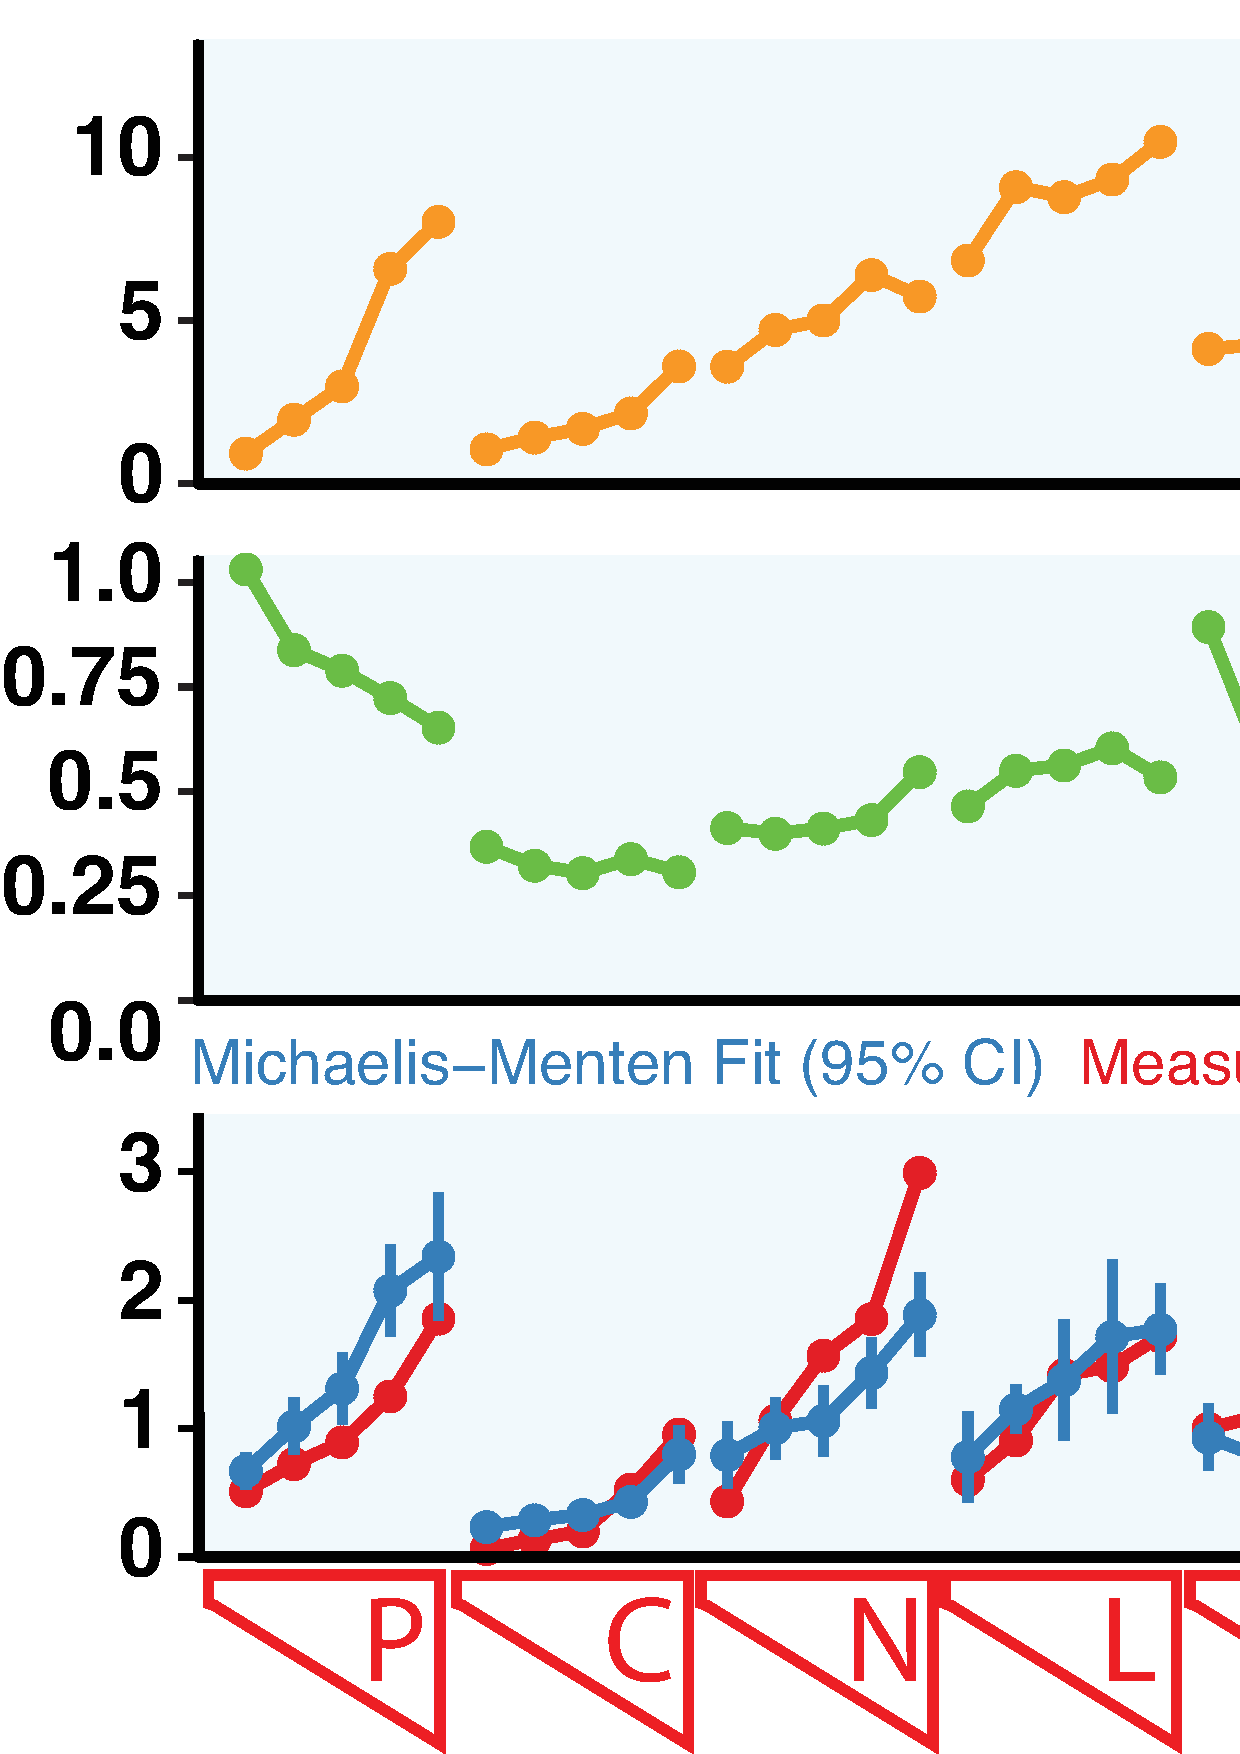
\includegraphics[width = 1\textwidth]{Figures/F3-MMkinetics.pdf}
\label{fig:TPI}
\end{figure}

\newpage

\begin{figure}[h!]
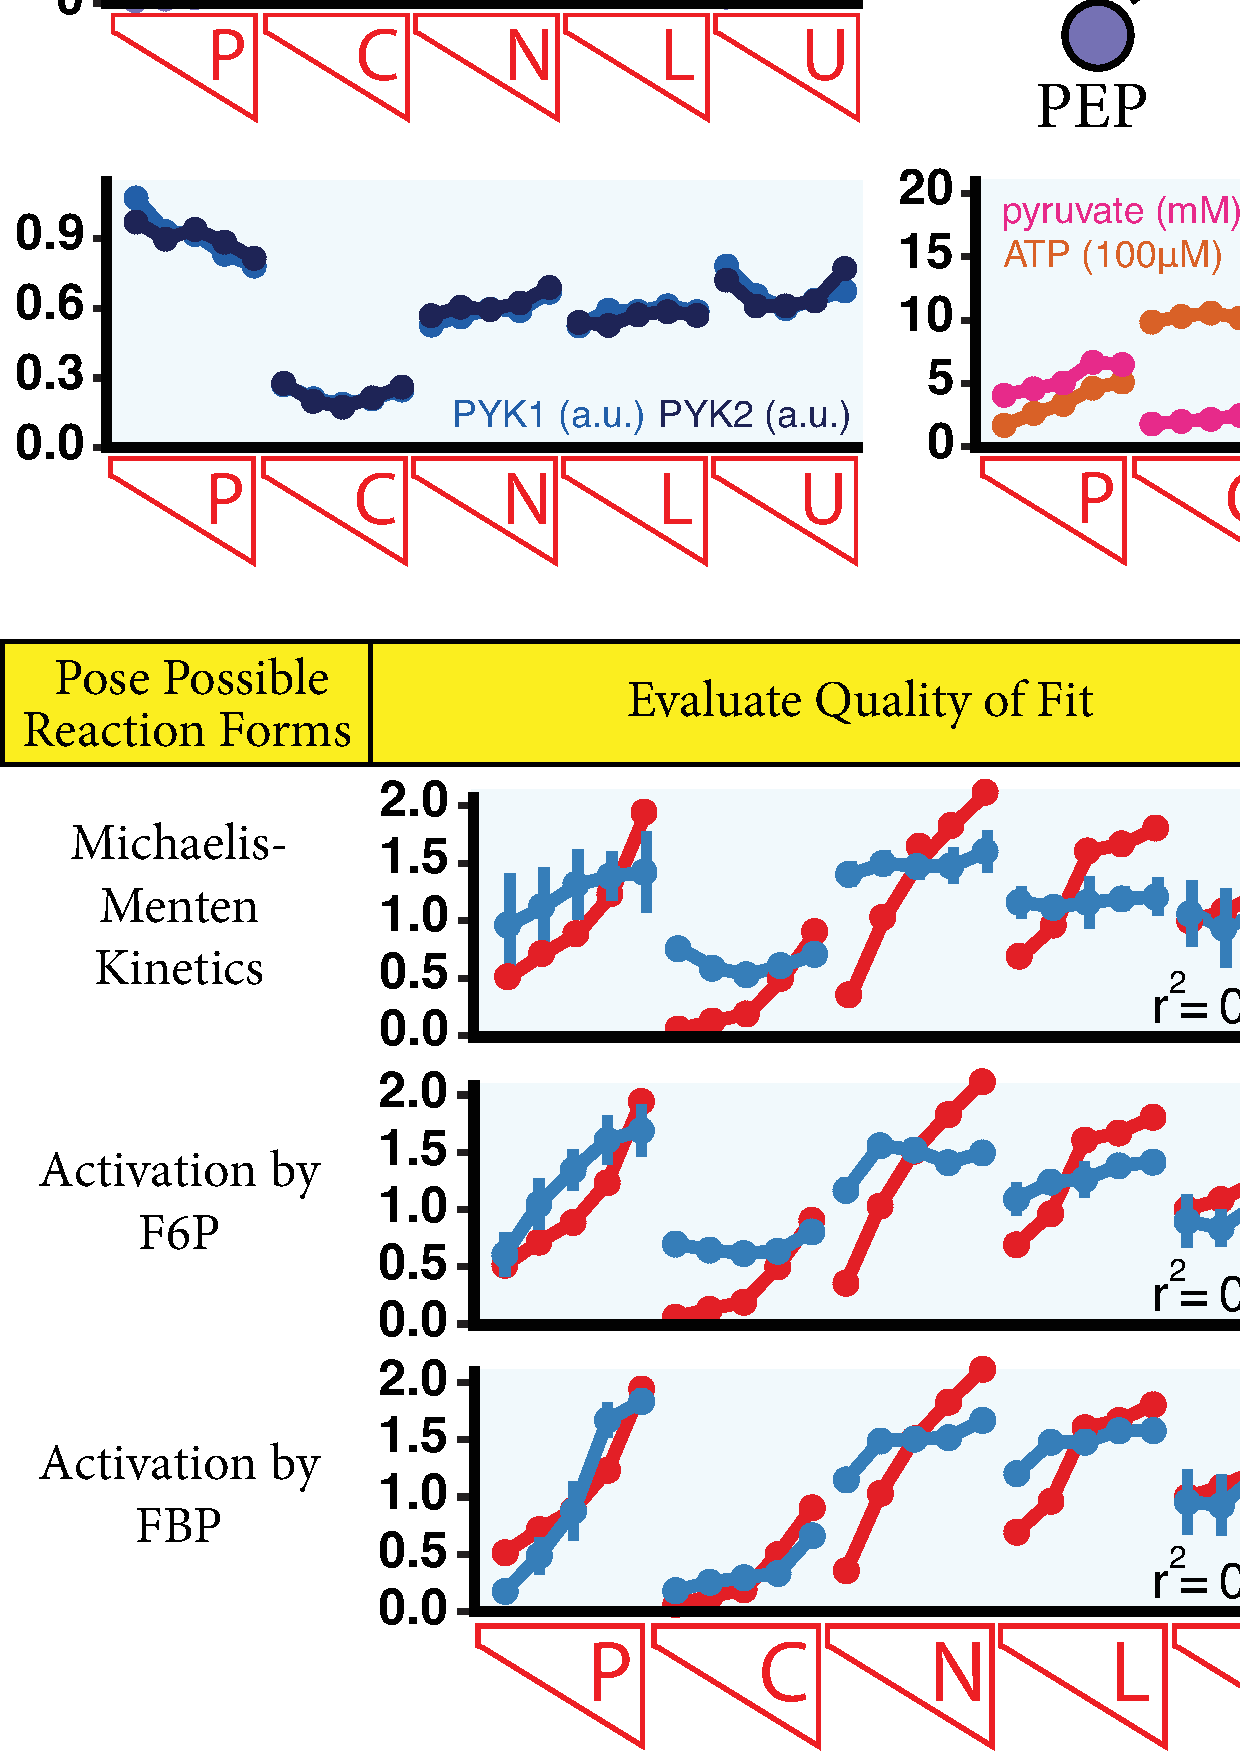
\includegraphics[width = 1\textwidth]{Figures/F4-identifyingRegulation.pdf}
\label{fig:PYK}
\end{figure}

\newpage

%\begin{figure}[h!]
%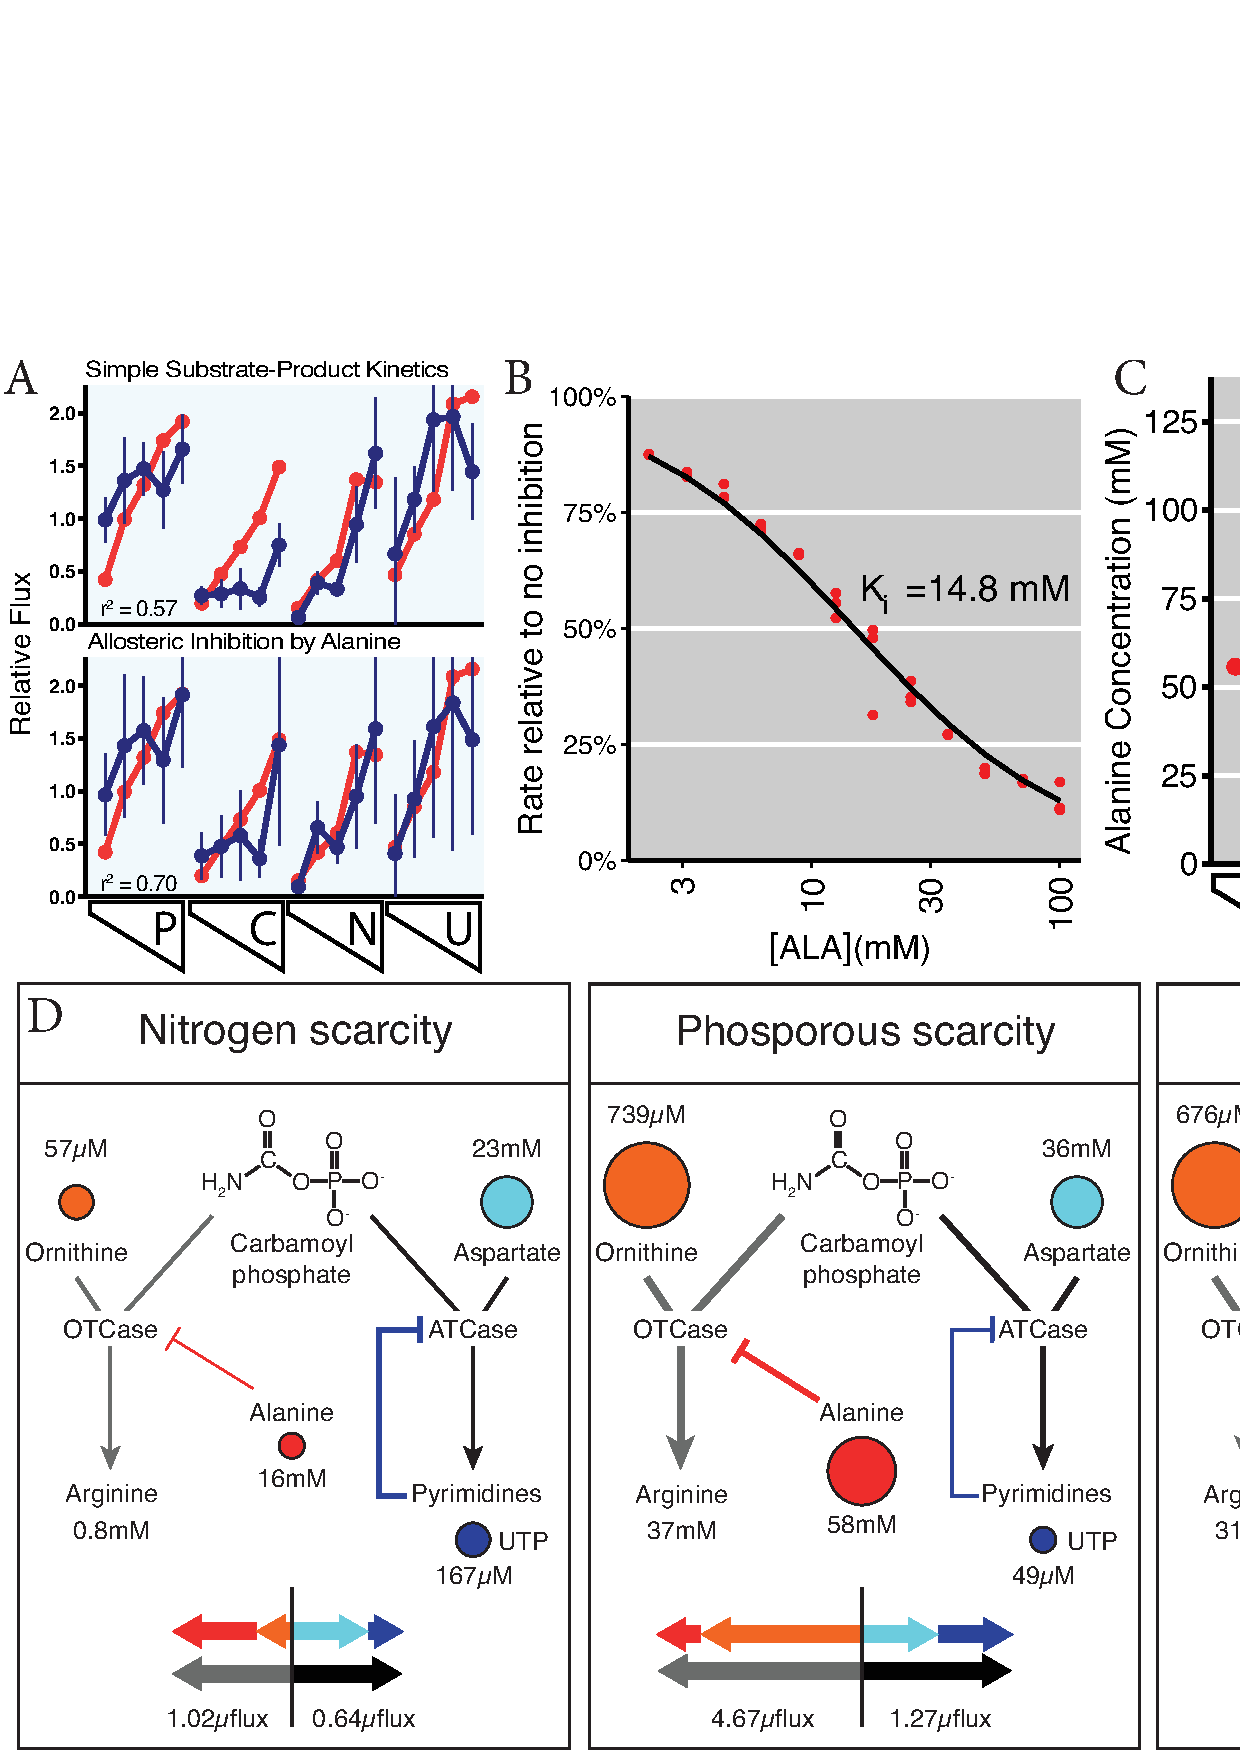
\includegraphics[width = 1\textwidth]{Figures/F4-OTCaseKinetics.pdf}
%\label{fig:OTCaseKinetics}
%\end{figure}


\newpage


\begin{figure}[h!]
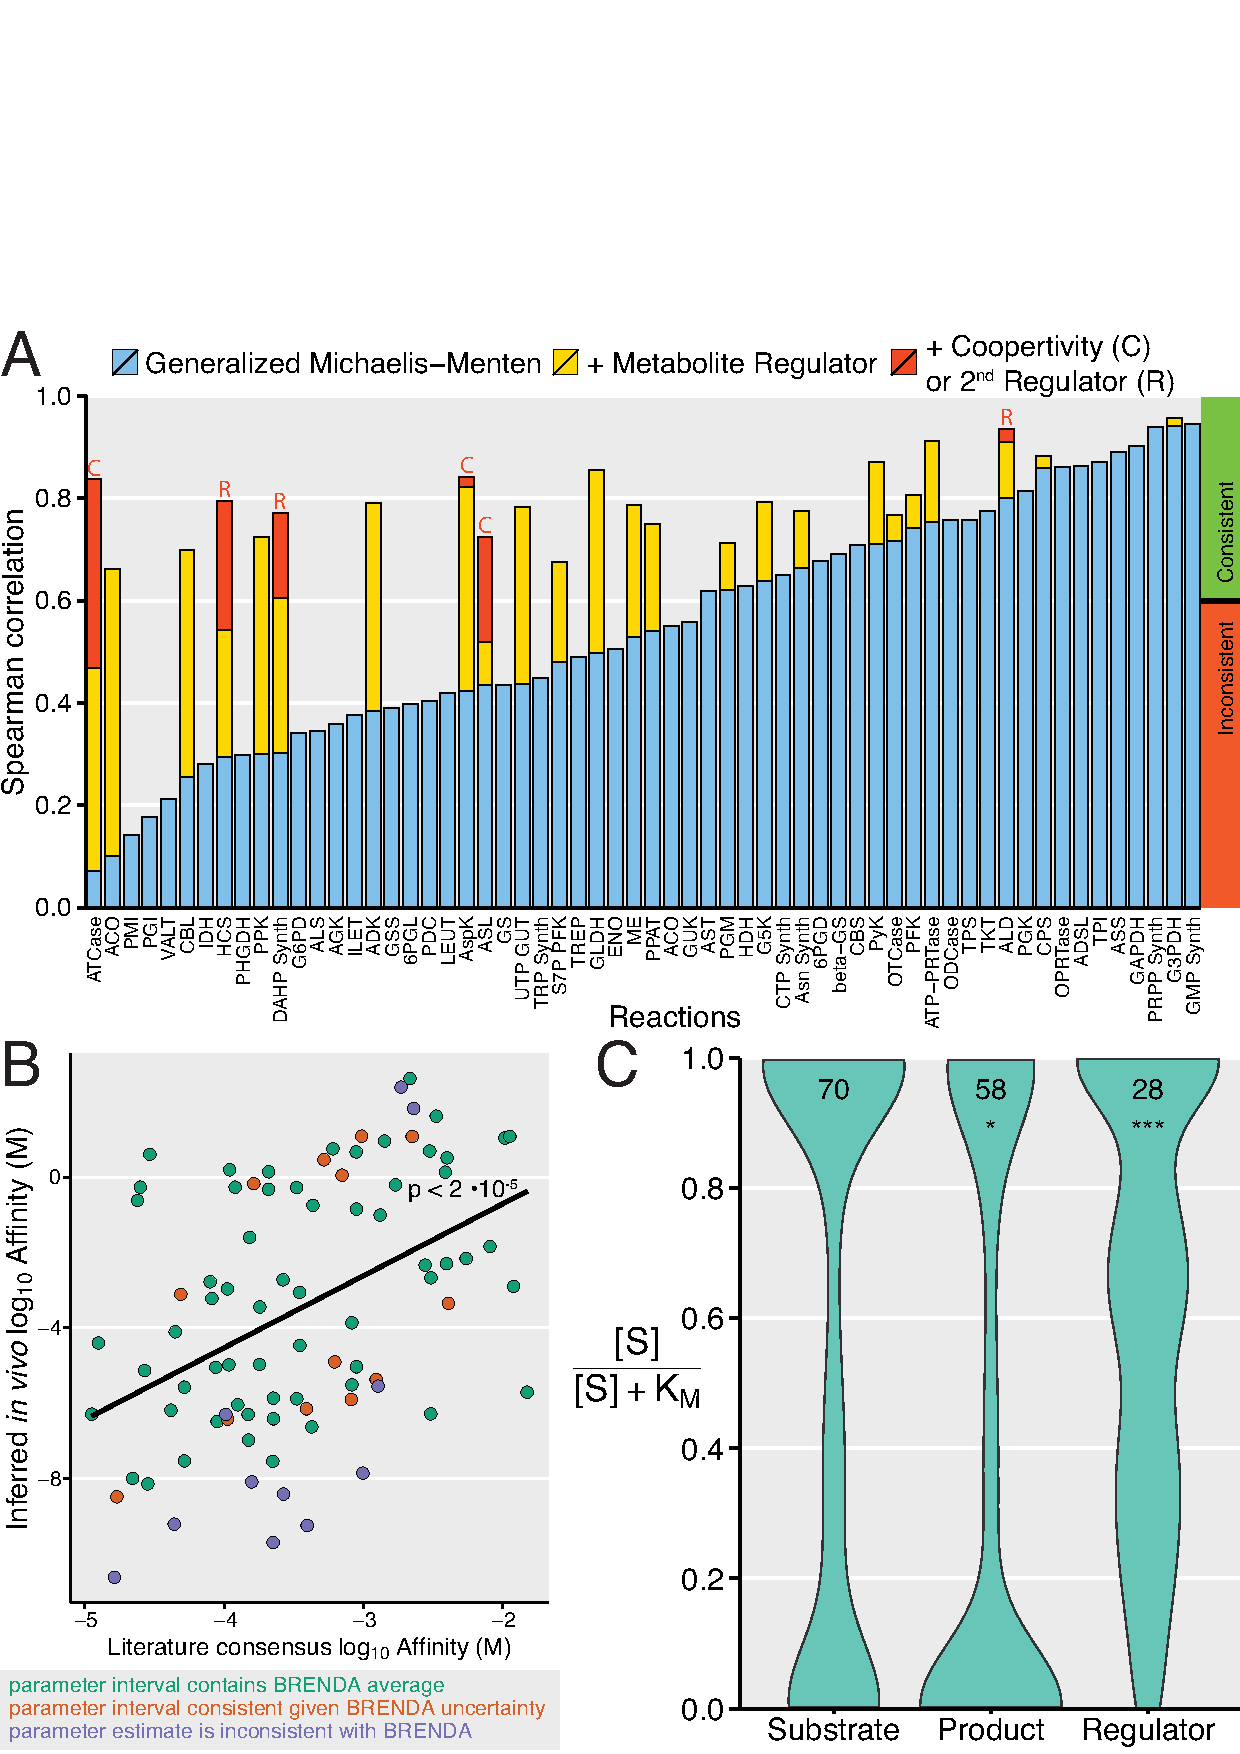
\includegraphics[width = 1\textwidth]{Figures/F5-performanceSummary.pdf}
\label{fig:allosteryFit}
\end{figure}

\newpage

\begin{figure}[h!]
\begin{center}
\includegraphics[width = 1\textwidth]{Figures/F6-MetabolicLeverage.pdf}
\label{fig:metabolicLeverage}
\end{center}
\end{figure}

\newpage
\cite{Fraenkel:2011wp}

\bibliographystyle{naturemag}
\bibliography{ROCAbiblio.bib}

\end{document} 
